\section{Tam giác hóa (Triangulation)}
\label{sec:triangulation}

Trong các phần trước, chúng ta đã thiết lập được ràng buộc epipolar và cách tìm các điểm tương ứng giữa hai ảnh. Tuy nhiên, các điểm tương ứng này vẫn chỉ tồn tại trong không gian 2D của ảnh.

Câu hỏi trung tâm lúc này là:

\begin{center}
	\textit{Làm thế nào để khôi phục lại vị trí thực sự của điểm trong không gian 3D?}
\end{center}

Triangulation chính là câu trả lời cho câu hỏi này. Nó là quá trình suy ra tọa độ 3D của một điểm từ các quan sát của nó trên nhiều ảnh.

\begin{center}
	\textit{Triangulation là bước “giải mã” hình học: từ nhiều phép chiếu 2D, ta tái tạo lại thực tại 3D.}
\end{center}

\subsection{Trực giác Hình học}
\label{subsec:triangulation_geometry}

Mỗi điểm ảnh tương ứng với một tia chiếu trong không gian 3D. Do đó:

\begin{itemize}
	\item $\mathbf{x}$ xác định một tia từ camera thứ nhất
	\item $\mathbf{x}'$ xác định một tia từ camera thứ hai
\end{itemize}

Trong trường hợp lý tưởng:

\begin{itemize}
	\item Hai tia này cắt nhau tại đúng điểm $\mathbf{X}$
\end{itemize}

\begin{center}
	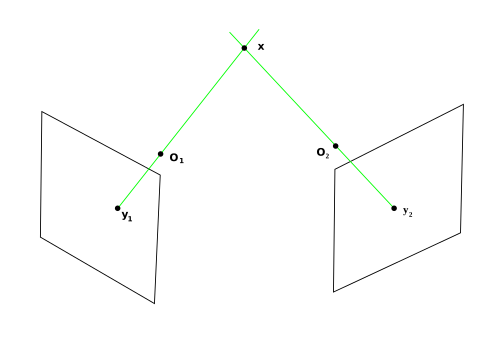
\includegraphics[width=0.8\textwidth]{images/triangulation_ideal.png}
	\captionof{figure}{Triangulation lý tưởng: hai tia chiếu từ hai camera cắt nhau tại điểm 3D thực sự.}
	\label{fig:triangulation_ideal}
\end{center}

Tuy nhiên, trong thực tế:

\begin{itemize}
	\item Dữ liệu luôn có nhiễu
	\item Các tia thường không giao nhau
\end{itemize}

\begin{center}
	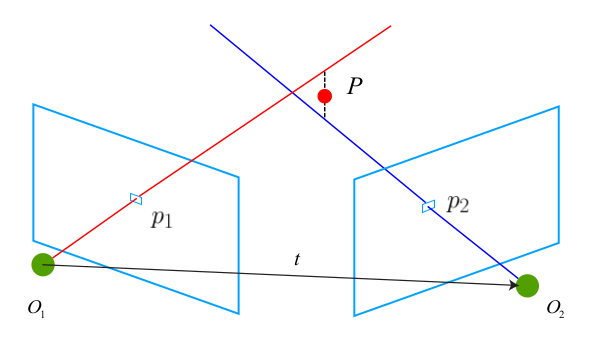
\includegraphics[width=0.8\textwidth]{images/triangulation_noisy.png}
	\captionof{figure}{Triangulation trong thực tế: hai tia không cắt nhau do nhiễu, dẫn đến bài toán tối ưu khoảng cách.}
	\label{fig:triangulation_noisy}
\end{center}

\begin{mdframed}[style=infobox]
	\textbf{Insight cốt lõi}
	
	Triangulation thực chất là một bài toán tối ưu: tìm điểm $\mathbf{X}$ “tốt nhất” phù hợp với nhiều tia chiếu không giao nhau.
\end{mdframed}

\subsection{Thiết lập Bài toán}
\label{subsec:triangulation_setup}

Cho:
\[
P, \quad P'
\]

và:
\[
\mathbf{x} \leftrightarrow \mathbf{x}'
\]

Ta cần tìm $\mathbf{X}$ sao cho:

\[
\mathbf{x} \sim P\mathbf{X}, \quad \mathbf{x}' \sim P'\mathbf{X}
\]

Đây là một bài toán overdetermined khi có nhiễu.

\subsection{Phương pháp Tuyến tính (Linear Triangulation)}
\label{subsec:linear_triangulation}

Từ:
\[
\mathbf{x} \sim P\mathbf{X}
\]

suy ra:

\[
\mathbf{x} \times (P\mathbf{X}) = 0
\]

Khai triển cho hai ảnh, ta thu được hệ:

\[
A \mathbf{X} = 0
\]

với $A \in \mathbb{R}^{4 \times 4}$.

\begin{mdframed}[style=infobox]
	\textbf{Insight}
	
	Triangulation tuyến tính có cấu trúc giống hệt DLT: tìm vector trong null space của một ma trận.
\end{mdframed}

Giải bằng SVD:
\begin{itemize}
	\item $\mathbf{X}$ là vector riêng ứng với singular value nhỏ nhất
\end{itemize}

\subsection{Vấn đề với Sai số Đại số}
\label{subsec:algebraic_error}

Phương pháp trên tối thiểu hóa:

\begin{itemize}
	\item Sai số đại số (algebraic error)
\end{itemize}

Nhưng điều này không có ý nghĩa hình học rõ ràng.

\begin{mdframed}[style=infobox]
	\textbf{Insight quan trọng}
	
	Một nghiệm có sai số đại số nhỏ chưa chắc có sai số hình học nhỏ. Đây là lý do phương pháp tuyến tính thường chỉ dùng làm khởi tạo.
\end{mdframed}

\subsection{Triangulation Tối ưu (Reprojection Error)}
\label{subsec:optimal_triangulation}

Ta định nghĩa:

\[
\min_{\mathbf{X}} \left( \|\mathbf{x} - \hat{\mathbf{x}}\|^2 + \|\mathbf{x}' - \hat{\mathbf{x}}'\|^2 \right)
\]

Đây là bài toán tối ưu phi tuyến.

Ý nghĩa:
\begin{itemize}
	\item $\mathbf{X}$ tốt nhất là điểm khi chiếu lại lên ảnh gần nhất với quan sát
\end{itemize}

\begin{mdframed}[style=infobox]
	\textbf{Diễn giải}
	
	Chúng ta không ép các tia phải giao nhau, mà tìm điểm khiến các phép chiếu khớp nhất với dữ liệu.
\end{mdframed}

\subsection{Midpoint Method}
\label{subsec:midpoint_method}

Hai tia trong không gian thường skew (không cắt nhau). Ta:

\begin{itemize}
	\item Tìm đoạn ngắn nhất nối hai tia
	\item Lấy trung điểm làm nghiệm
\end{itemize}

Ưu điểm:
\begin{itemize}
	\item Có trực giác hình học rõ ràng
\end{itemize}

Nhược điểm:
\begin{itemize}
	\item Không tối ưu theo reprojection error
\end{itemize}

\subsection{Điều kiện Hình học và Conditioning}
\label{subsec:conditioning}

Độ chính xác của triangulation phụ thuộc mạnh vào góc giữa hai tia.

\begin{itemize}
	\item Góc lớn → giao cắt rõ → ổn định
	\item Góc nhỏ → gần song song → sai số lớn
\end{itemize}

\begin{mdframed}[style=infobox]
	\textbf{Baseline}
	
	Baseline lớn giúp cải thiện độ chính xác chiều sâu, nhưng quá lớn có thể gây khó khăn cho matching.
\end{mdframed}

\paragraph{Error amplification}

Một sai số nhỏ trong pixel có thể dẫn đến sai số lớn trong $\mathbf{X}$ nếu:
\begin{itemize}
	\item hai tia gần song song
\end{itemize}

\subsection{Cheirality Constraint}
\label{subsec:cheirality}

Một nghiệm hợp lệ phải thỏa:

\begin{itemize}
	\item $\mathbf{X}$ nằm trước cả hai camera
\end{itemize}

\begin{mdframed}[style=infobox]
	\textbf{Insight}
	
	Cùng một cặp điểm có thể cho nhiều nghiệm toán học, nhưng chỉ nghiệm thỏa điều kiện cheirality mới có ý nghĩa vật lý.
\end{mdframed}

\subsection{Mối liên hệ với Epipolar Geometry}
\label{subsec:triangulation_epipolar}

Pipeline đầy đủ:

\begin{itemize}
	\item Fundamental matrix → ràng buộc epipolar
	\item Matching → tìm correspondences
	\item Triangulation → khôi phục $\mathbf{X}$
\end{itemize}

\begin{mdframed}[style=infobox]
	\textbf{Insight hệ thống}
	
	Epipolar geometry giảm không gian tìm kiếm, còn triangulation biến kết quả tìm kiếm thành cấu trúc 3D.
\end{mdframed}

\subsection*{Kết luận}
\label{subsec:triangulation_conclusion}

Triangulation là bước hoàn tất chuỗi suy luận hình học:

\begin{itemize}
	\item từ điểm ảnh → tia chiếu
	\item từ hai tia → ước lượng điểm 3D
\end{itemize}

Mặc dù ý tưởng cơ bản đơn giản, việc thực hiện chính xác đòi hỏi:

\begin{itemize}
	\item dữ liệu tốt
	\item cấu hình camera hợp lý
	\item tối ưu phi tuyến
\end{itemize}

Hiểu rõ triangulation không chỉ là hiểu một thuật toán, mà là hiểu cách thông tin hình học được tái tạo từ dữ liệu không hoàn hảo.

\section*{Tài liệu tham khảo}
\begin{itemize}
	\item[1] Hartley, R., \& Zisserman, A. (2003). \textit{Multiple View Geometry in Computer Vision}.
	\item[2] Ma, Y. et al. (2004). \textit{An Invitation to 3-D Vision}.
	\item[3] Faugeras, O. (1993). \textit{Three-Dimensional Computer Vision}.
\end{itemize}